\apendice{Documentación técnica de programación}

\section{Introducción}
En esta sección describiré como está estructurado el proyecto, que es necesario para poder ejecutarlo desde cualquier ordenador y lo más relevante a la hora de crearlo.
\section{Estructura de directorios}
La estructura de los ficheros alojados en el \href{https://github.com/jgo0038/TFG-Reserva-aulas-informatica}{repositorio de GitHub} es la siguiente:
\begin{itemize}
    \item \textbf{ReservaAulas:} Contiene el proyecto y el entorno virtual y configuraciones.
    \begin{itemize}
        \item \textbf{.vscode:} Contiene la configuración para ejecutar en \textit{debug} desde \textit{VSCode}.
        \item \textbf{azureEnv:} Entorno virtual creado para el proyecto.
        \item \textbf{reservaAulas\_app:} Contiene el proyecto principal. Dentro se encuentran los ficheros que contienen la funcionalidad del proyecto. También alberga las conexiones con la base de datos, con Azure y con la API.
        \begin{itemize}
            \item \textbf{static:} Contiene imágenes, bibliotecas y ficheros javascript que se usan en el proyecto.
            \begin{itemize}
                \item \textbf{css:} Estilos de Bootstrap y algunos propios para HTML.
                \item \textbf{img:} Imágenes del proyecto.
                \item \textbf{js:} Ficheros JavaScript de Bootstrap.
            \end{itemize}
            \item \textbf{templates:} Contiene los ficheros de la parte de la vista del proyecto.
        \end{itemize}
        \item \textbf{requirements.txt:} Contiene los requisitos a instalar dentro del entorno virtual para el funcionamiento del proyecto.
        \item \textbf{startup:} Fichero para hacer el deploy a Azure.
    \end{itemize}
\end{itemize}
\section{Manual del programador}
\subsection{Estructura del proyecto}
En esta sección se explican las distintas entidades del proyecto y con qué finalidad se han creado. Se trata de explicar los ficheros del proyecto desde el punto de vista del programador para que se entienda el código para futuras mejoras o análisis del mismo. A continuación enumero y explico los ficheros usados:
\begin{itemize}
    \item \textbf{reservaAulas/azureEnv}: Entorno virtual creado para instalar las dependencias necesarias del proyecto.
    \item \textbf{reservaAulas/reservaAulas\_app}: Contiene todo el código del proyecto.
    \begin{itemize}
        \item \textbf{static}: Contiene las carpetas de 'css', 'img' y 'js'. En ellas se guardan los estilos de \textit{Bootstrap}, las imágenes que utilizamos y los archivos \textit{JavaScript} necesarios para \textit{Bootstrap} o alguno propio, respectivamente.
        \item \textbf{templates}: Contiene el código \textit{HTML}, \textit{Jinja2} y \textit{JavaScript} que crean las interfaces que verá el usuario.
        \item \textbf{reservaAulas\_app}: Contiene el código que maneja la lógica de la aplicación, proporciona y recoge los datos desde la API y base de datos.
    \end{itemize}
\end{itemize}

\begin{itemize}
    \item \textbf{reservaAulas/.deployment:} fichero generado al realizar el deploy en Azure.
    \item \textbf{log\_web\_app.log:} fichero generado para encontrar errores al hacer el deploy.
    \item \textbf{reservaAulas/createTablesSQLServer.sql:} fichero con el código correspondiente para generar las tablas y relaciones entre ellas necesarias para el proyecto.
    \item \label{requirements} \textbf{reservaAulas/requirements.txt:} fichero generado con las bibliotecas necesarias a instalar en el entorno virtual para que funcione la aplicación.
    \item \textbf{reservaAulas/startup.py:} fichero generado para ejecutar desde Azure.
    \item \textbf{reservaAulas/.vscode/launch.json:} configuración para ejecutar el proyecto desde el VSCode en un entorno virtual.
    \item \textbf{reservaAulas/reservaAulas\_app/\_\_init\_\_.py:} creación de la app de Flask e instancia de la base de datos y el cifrado csrf.
    \item \textbf{reservaAulas/reservaAulas\_app/config.py:} configuración de la aplicación con las claves iniciales de Azure para el uso de la API de Outlook y creación de los permisos.
    \item \textbf{reservaAulas/reservaAulas\_app/forms.py:} creación de los formularios que se utilizan en las páginas de la aplicación.
    \item \textbf{reservaAulas/reservaAulas\_app/getSQLData.py:} fichero con llamadas a la base de datos para ahorrar código en el fichero views.py.
    \item \textbf{reservaAulas/reservaAulas\_app/models.py:} modelos utilizados en base de datos en local.
    \item \textbf{reservaAulas/reservaAulas\_app/oauth\_helpers.py:} funciones que llaman a la API de Outlook para recoger, enviar, borrar o actualizar datos.
    \item \textbf{reservaAulas/reservaAulas\_app/odbctest:} conexión mediante pyodbc con la base de datos subida a Azure.
    \item \textbf{reservaAulas/reservaAulas\_app/views.py:} fichero que contiene la funcionalidad del servidor, llama a las funciones de otros ficheros para obtener datos y los envía al cliente.
    \item \textbf{reservaAulas/reservaAulas\_app/webapp.py:} fichero creado para la creación de la estructura pedida por VSCode y Azure.
    \item \textbf{reservaAulas/reservaAulas\_app/templates/anadirAulas.html:} fichero que contiene lo que verá el cliente a la hora de añadir un aula.
    \item \textbf{reservaAulas/reservaAulas\_app/templates/anadirPropietarios.html:} fichero que contiene la parte del cliente al intentar crear un propietario nuevo.
    \item \textbf{reservaAulas/reservaAulas\_app/templates/auditoria.html:} fichero que contiene el código para que el cliente pueda ver la tabla de auditorías.
    \item \textbf{reservaAulas/reservaAulas\_app/templates/errorModificarEvento.html:} fichero que permite al cliente ver el mensaje de error al intentar modificar un evento y que se solapen las horas con algún evento existente.
    \item \textbf{reservaAulas/reservaAulas\_app/templates/errorPermisos.html:} fichero que muestra al cliente un mensaje de error cuando se le ha hecho propietario de un calendario pero no se le han dado los permisos manualmente y no puede acceder a sus funcionalidades.
    \item \textbf{reservaAulas/reservaAulas\_app/templates/events.html:} página que pide al cliente las características de los eventos que se quieren visualizar .
    \item \textbf{reservaAulas/reservaAulas\_app/templates/eventsTable.html:} contiene el código de la parte del cliente que permite ver la tabla con los eventos que coincidan con las especificaciones pasadas, permite modificar y borrar los eventos si se tiene permisos.
    \item \textbf{reservaAulas/reservaAulas\_app/templates/home.html:} página de inicio de sesión y página principal si ya se ha iniciado sesión.
    \item \textbf{reservaAulas/reservaAulas\_app/templates/mensajePropietario.html:} fichero que permite al cliente ver el mensaje recordatorio al administrador para que asigne los permisos manualmente cuando crea un nuevo propietario o modifica el propietario de un aula.
    \item \textbf{reservaAulas/reservaAulas\_app/templates/navBar.html:} contiene código común para la barra de navegación superior y la franja inferior, heredan de ella para ahorrar código duplicado.
    \item \textbf{reservaAulas/reservaAulas\_app/templates/reservar.html:} fichero que contiene el código para mostrar al cliente la página desde la que pueden realizar una reserva de un aula.
    \item \textbf{reservaAulas/reservaAulas\_app/templates/showEventsTable.html:} contiene la tabla de eventos que se muestra al elegir la opción de ver los eventos de un aula que se va a reservar desde la ventana de reservar.
    \item \textbf{reservaAulas/reservaAulas\_app/templates/verAulas.html:} fichero que contiene el código que ve el cliente al ver la lista de aulas.
    \item \textbf{reservaAulas/reservaAulas\_app/templates/verPropietarios:} página que muestra una tabla en la que se ven los propietarios existentes.
\end{itemize}


\section{Compilación, instalación y ejecución del proyecto}
En esta sección será explicada la compilación, lo necesario para realizar la instalación correctamente y la forma de ejecutar el proyecto. Primeramente se explican los pasos que se tuvieron que realizar para poder registrar la aplicación en Microsoft Azure y permitir el acceso a el presente proyecto mediante el login de Microsoft que haremos funcionar al registrar la aplicación previamente.\newline

Comentando el uso de la API de Microsoft para acceder a los datos de Outlook y poder habilitar un inicio de sesión bajo Microsoft, hubo que registrar la aplicación en Azure Active Directory, para ello fueron seguidos estos pasos:
\begin{itemize}
    \item Acceder al centro de administración de Azure Active Directory.
    \item Acceder al apartado registro de aplicaciones y crear un nuevo registro.
    \item Una vez ahí dentro, se pedirá rellenar unos campos con el nombre de la aplicación, cuentas que accederán y lo más importante, la dirección URL de redirección al iniciar sesión mediante Outlook.\newline
    \imagen{AzureAutenticacion1}{URL de respuesta de nuestra aplicación}
    \item Una vez se ha creado, recogemos el ID de la aplicación obtenido, que se utilizará para obtener el secreto del cliente, que solamente se mostrará una vez y será necesario para el resto del proyecto. Para obtenerlo se accede a certificados y secretos, se escribe un nombre para registrar la aplicación y se elige una duración límite para que expire el secreto que se recibirá y haya que pedirlo de nuevo, de esta forma se obtiene dicho secreto desde Azure Active Directory.
\end{itemize}
Esto está especificado en el tutorial de Microsoft\cite{pythonMicrosoftGraph}. \newline
Una vez registrada la aplicación disponemos del código secreto, que no se volverá a repetir, y del identificador de la aplicación que se ve en la figura \ref{fig:AzureAutenticacion2}. Hubo que seguir una serie de pasos para incluirlo en el código y hacer que funcionara:
\imagen{AzureAutenticacion2}{Código de aplicación de Azure Active Directory}
\begin{itemize}
    \item Agregar al fichero 'config.py' el secreto recibido, el identificador de la aplicación de Azure y la ruta a la que redirigir una vez se ha logeado. Con esto se configura nuestro proyecto para la conexión con la aplicación registrada en Azure que se ha realizado en los pasos anteriores (ver figura \ref{fig:AzureAutenticacion}) .
    \imagen{AzureAutenticacion}{Código incluyendo la aplicación de Azure Active Directory}
    \item Agregar al fichero 'config.py' el código con los permisos de Outlook que se van a proporcionar al usuario que acceda, en este proyecto son los siguientes: leer el usuario, lectura de calendarios y calendarios compartidos, escritura de calendarios y calendarios compartidos, acceso al email, acceso offline,
    \item Crear en el ficheero 'oauth\_helpers.py' unas funciones con llamadas a la API REST para obtener un token de inicio de sesión y otro para refrescarle. Esto servirá para cada sesión de cada usuario diferente.
\end{itemize}
Una vez se creó este primer código que permitía acceder mediante el inicio de sesión de Outlook a la página que especificamos en Azure Active Directory como URL de redirección, se pudo empezar a trabajar con llamadas a la API REST para obtener información sobre los calendarios del usuario y sus eventos.\newline

La descarga del proyecto desde GitHub se puede realizar en:\newline
\url{https://github.com/jgo0038/TFG-Reserva-aulas-informatica}\newline
En el entorno de desarrollo, lo primero que hay que tener es una instalación de \textit{Python} y un entorno virtual, si no se tiene, habrá que crearlo de forma sencilla con el siguiente comando\newline
\textbf{\textit{python3 -m venv /path/to/new/virtual/environment}}\newline o utilizar directamente el que se descarga con el repositorio.
\newline
 Una vez se tenga esto creado, se activa el entorno virtual donde instalaremos las dependencias necesarias, como ya se explicó antes, especificadas en el fichero 'requirements.txt' (ver \ref{requirements}). Este fichero sirve para realizar una instalación muy simple con un sencillo comando: \newline
 \textbf{\textit{\$ pip install -r requirements.txt }} \newline
Con este comando se instalarán las bibliotecas necesarias para esta versión usada dentro de nuestro entorno virtual. El siguiente paso será la compilación y ejecución del proyecto. \newline

\label{ConexionDB}
Para la ejecución de nuestra aplicación web, se necesita un servidor web que haga de host para la base de datos. Como ya se ha visto en otros apartados, se ha utilizado Azure, por lo que la conexión con la base de datos ha sido particularizada para este servidor en concreto (ver fichero 'reservaAulas/reservaAulas\_app/odbctest.py') que contiene el nombre del servidor, de la base de datos, usuario, contraseña, puerto de Azure (1433) y driver para conectarse exactamente a esta base de datos de SQL Server alojada en Azure. Para que funcione con estas mismas configuraciones, hay que crear la base de datos con los mismos nombres que se muestran en la siguiente imagen, o bien adaptarlo a otra base de datos.\newline
\imagen{ConexionDBAzure1}{Código para conectar con la BD de Azure}
\newline Si se quisiera realizar en un servidor instalado en local, se tendría que cambiar la conexión y ajustarla al servidor utilizado. Azure restringe el acceso a las bases de datos desde otros ordenadores mediante la configuración del firewall, en el que se introducen las direcciones IP que pueden acceder a esta base de datos (actualmente solo puede realizarse desde el equipo utilizado por el alumno).\newline
\imagen{ConexionDBAzure2}{Restricción de direcciones IP para la conexión}
\newline
Debido a esta particularidad de la configuración del firewall de la base de datos, para poder acceder al proyecto como desarrollador se necesita crear una base de datos con las mismas relaciones que las especificadas en los diagramas y cambiar la conexión del fichero 'odbctest.py' para conectarse a ella, o bien añadir la IP al firewall de la base de datos de Azure.\newline
Si no se tiene acceso a la base de datos, se puede ejecutar desde el servidor de Azure al que está subida la aplicación accediendo desde el siguiente enlace \url{https://reservaaulas.azurewebsites.net} como cliente, esto lo veremos en el manual de usuario.\newline
Si se dispone de acceso a la base de datos, se podrá realizar una ejecución en local accediendo a la base de datos del servidor de Azure, para ello propongo dos opciones:\newline
Si se trabaja con VSCode (es el caso del alumno) los pasos a seguir son los siguientes:
\begin{itemize}
    \item Activar el entorno virtual.
    \item Ejecutar desde el modo debug que proporciona VSCode, ya está configurado en 'reservaAulas/.vscode/launch.json' el fichero que se tiene que ejecutar en el entorno para que el proyecto se ponga en marcha en el puerto elegido, que es el 5000.
    \item Acceder a la aplicación desde nuestro localhost.
\end{itemize}
Si por otro lado, se quiere ejecutar desde cualquier otro lugar, hay que establecer manualmente las configuraciones que se acaban de comentar. Esto se hace de la siguiente forma:
\begin{itemize}
    \item Activar el entorno virtual.
    \item Establecer la variable de entorno 'FLASK\_APP', el comando para hacerlo es el siguiente:\newline
    \textbf{\textit{\$ set FLASK\_APP=reservaAulas\_app.webapp}}\newline
    Si no utiliza Windows, use export en vez de set.
    \item El siguiente paso es ejecutar el proyecto, para ello ejecutamos la siguiente línea:\newline
    \textbf{\textit{python -m flask run}}
    \item Acceder a la aplicación desde nuestro localhost.
\end{itemize}
Una vez se tiene acceso a la aplicación, si la ejecutamos también logeados como el administrador necesitaremos acceder a Outlook para poder compartir los calendarios con los propietarios. A continuación dejo la serie de pasos a seguir para compartir manualmente un calendario con un responsable:
\begin{itemize}
    \item Iniciar sesión con la cuenta administrador del proyecto (las credenciales se facilitan en el archivo de texto 'EnlacesInteres.txt' adjunto al proyecto ).
    \item Acceder a la pestaña de calendarios de Outlook. \newline
   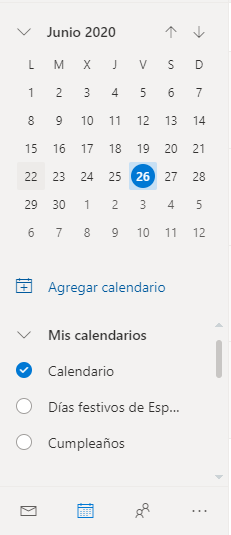
\includegraphics[scale=0.8]{CompartirCalendario}{Pestaña de calendarios}
    \item Pinchar en los tres puntos del calendario a compartir y elegir la opción de 'Uso compartido y permisos'.\newline
    \imagen{CompartirCalendario2}{Uso compartido y permisos}
    \item Escribir la dirección de correo del propietario con el que se quiere compartir el calendario, o seleccionar el icono de la papelera en el caso de querer quitar el permiso a algún propietario.\newline
    \imagen{CompartirCalendario3}{Compartir o borrar}
\end{itemize}
\section{Pruebas del sistema}
En esta sección realizaré pruebas manuales de los casos de uso sobre el sistema comprobando que todo funciona correctamente.
\tablaSmallSinColores{Pruebas manuales propietario}{p{7cm} p{7cm} }{pruebasmanuales}{
  \multicolumn{1}{p{3.25cm}}{\textbf{Descripción}} & \textbf{Respuesta{}}\\
 }
 {
  Iniciar sesión introduciendo los datos de una cuenta de Outlook  & {Se accede a la aplicación}\\\hline
  Consultar eventos de aulas &{Se muestra la tabla con los eventos que coincidan con las especificaciones.}\\\hline
  Consultar eventos de aulas sin completar los campos obligatorios & {Se pide que se rellenen los campos vacíos que sean obligatorios.}\\\hline
  Modificar un evento & {Se vuelve a la pantalla anterior y se muestra un mensaje de éxito en la modificación. Se modifica la información en el evento del calendario correspondiente de Outlook también.}\\\hline
  Modificar un evento cambiando la hora a unas ya ocupadas & {Se muestra una pantalla con un mensaje indicando que las horas están ocupadas y se ofrece la posibilidad de volver atrás.}\\\hline
  Borrar más de un evento seleccionado y aceptando la confirmación de los deseados & {Se muestra un mensaje de éxito en un cuadro de diálogo y se pide confirmación para mantenerse en la misma página con los mismos datos. Se borran los eventos de los calendarios de Outlook también.}\\\hline
  Realizar reserva introduciendo todos los campos correctamente y en fechas que estén libres & {Se queda en la misma página con el mismo formulario relleno que acabas de reservar y un mensaje en la parte inferior de éxito en la reserva. Se crea el evento en el calendario correspondiente de Outlook y se envía un email de notificación al profesor que solicitó la reserva.}\\\hline
  Realizar reserva introduciendo algún campo en blanco  & {Se pide que se rellenen los campos vacíos.}\\\hline
  Realizar reserva introduciendo fechas ya reservadas  & {Se queda en la misma página con el mismo formulario relleno que acabas de reservar y un mensaje en la parte inferior de error en las horas de la reserva.}\\\hline
  Consultar aulas especificando el edificio del que se quieren ver & {Se muestra una tabla con las aulas del edificio seleccionado y sus características.}

  }
 En esta tabla realizaré pruebas con funcionalidades únicamente del administrador.
 \tablaSmallSinColores{Pruebas manuales administrador}{p{7cm} p{7cm} }{pruebasmanuales}{
  \multicolumn{1}{p{3.25cm}}{\textbf{Descripción}} & \textbf{Respuesta{}}\\
 }
 {
  Modificar aulas & {Se vuelve a la página anterior y se muestra un mensaje por pantalla de éxito en la modificación.}\\\hline
  Modificar aulas cambiando el propietario & {Se muestra una pantalla en la que se lee un mensaje recordando al administrador de dar enviar el permiso de editar el calendario manualmente desde Outlook.}\\\hline
  Borrar un aula aceptando la confirmación & {Salta un cuadro de diálogo en el que se indica que se ha borrado correctamente el aula y se vuelve a la página anterior.}\\\hline
  Crear un aula con espacios en blanco en el formulario & {Se pide rellenar los espacios vacíos dejados.}\\\hline
  Crear un aula correctamente & {Se mantiene en la misma página mostrando el formulario completo y un mensaje en la parte inferior de éxito al crear el aula.}\\\hline
  Añadir un propietario sin completar todos los campos &
  {Se pide que se rellenen los campos vacíos}\\\hline
  }